\chapter[$^{14}$N ESEEM Data of Hox from CpI.]{Three-Pulse $^{14}$N ESEEM Data of H$_{ox}$ from CpI.}

The following three-pulse ESEEM data was taken by following the fusca-colored resonance roadmap of Fig.~\ref{fig:xTalFeFe}A in Chapter 6. Herein, the $\tau$ starts at 200~ns, $t_1$ starts at 300~ns with 256 24~ns steps, and $\pi$-pulse is 80~ns at a microwave power of 7~mW. A total of 16 $\tau$ values are taken from 200~ns to 424~ns over an 18 minute collection time per trace.

\begin{figure}[ht]
 \centering
 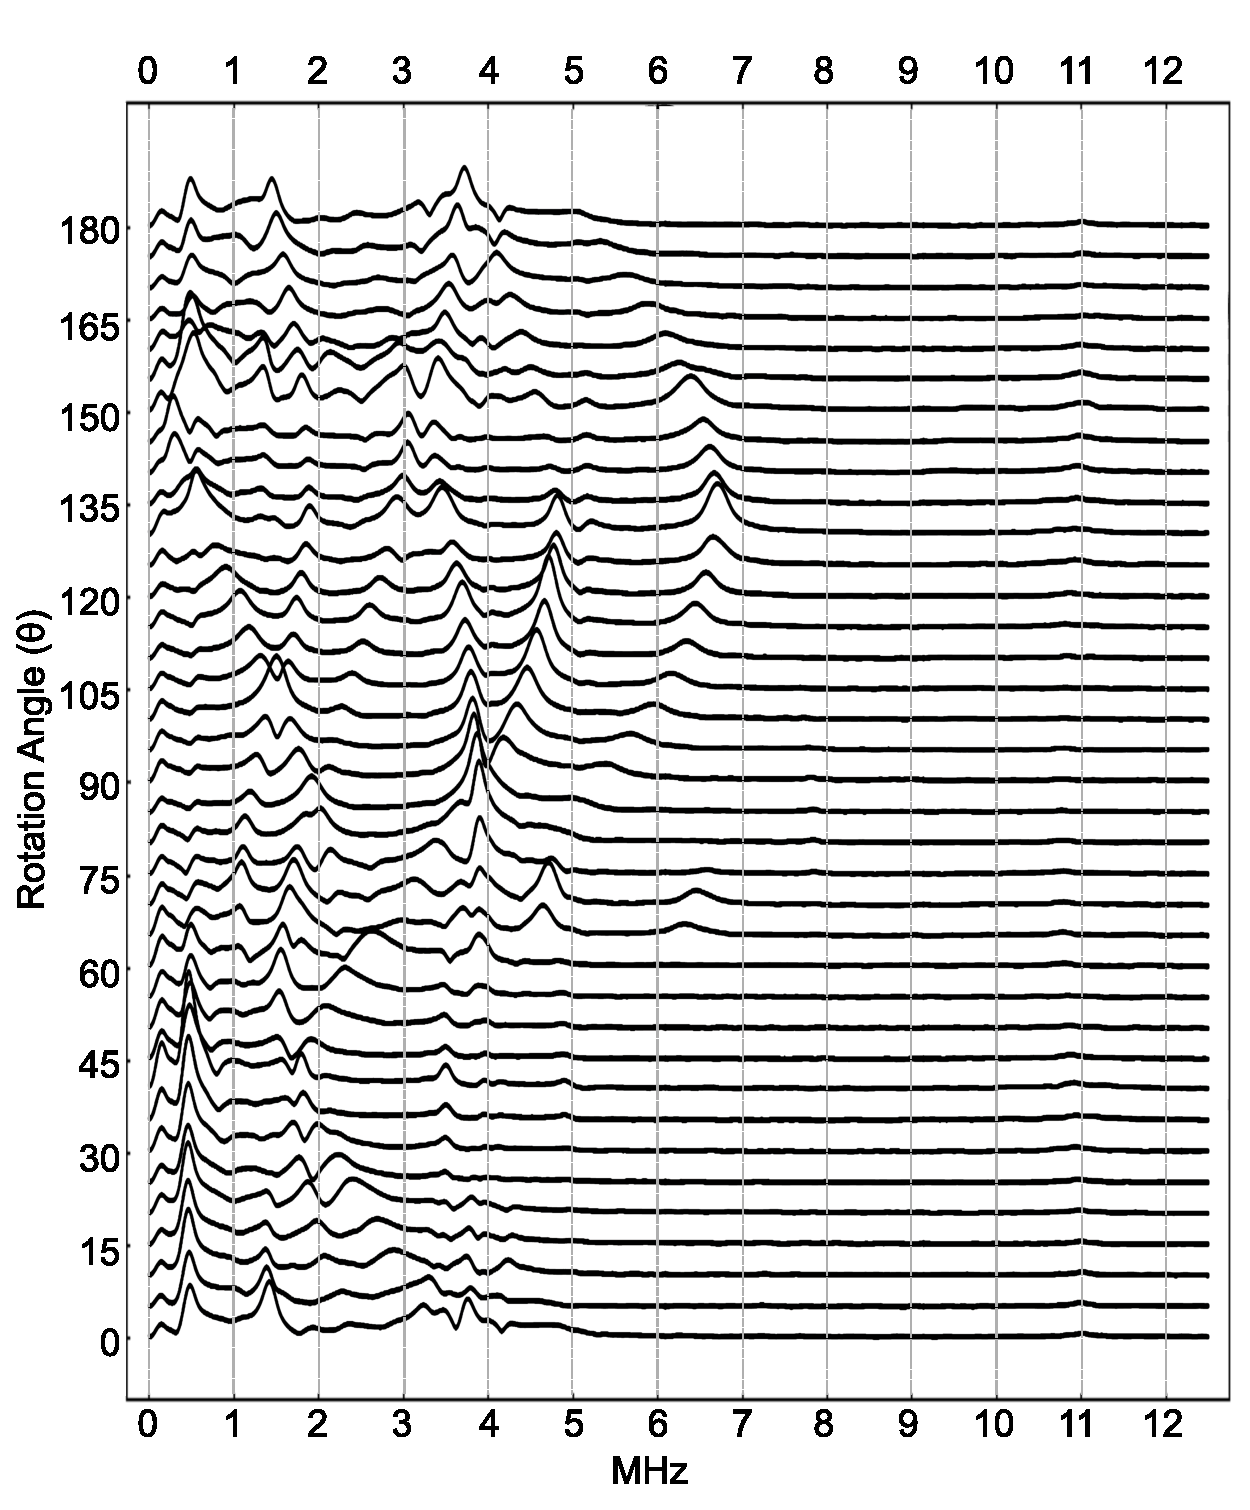
\includegraphics[width=0.85\textwidth]{Kapitel/Appendix/ESEEMFirstPeakA.eps}
 \caption[Preliminary Three-Pulse $^{14}$N ESEEM Data of H$_{ox}$ from CpI]{Three-pulse $^{14}$N ESEEM data from CpI in the H$_{ox}$ stable intermediate.}
 \label{fig-E:ESEEM}
\end{figure}

The data in Fig.~\ref{fig-E:ESEEM} represents the state-of-the-art signal-to-noise ratio for the study of protein single-crystals with volumes less than 3~nl. Further analysis is underway.

